\subsection{Connectivity chronology and threats to the comparison}
\label{app:connectivity_audit}

The connectivity record is useful both for defining exposure and for assessing the comparison series. Network traffic is not itself a measure of GitHub production, and a provider-level disruption need not affect every account in a country. The following review records documented events within the May 1--September 4 observation period. Absence from these non-exhaustive reports is not evidence of uninterrupted connectivity.

\begin{table}[htbp]
\centering\small
\caption{Documented connectivity events relevant to the analysis}
\label{tab:evidence_connectivity}
\begin{threeparttable}
\begin{tabular}{@{}p{.14\textwidth}p{.16\textwidth}p{.36\textwidth}p{.25\textwidth}@{}}
\toprule
Country & Date (2024) & Documented event & Implication \\
\midrule
Bangladesh & July 18 & Near-zero national traffic around 15:00 UTC \citep{belson2024} & Daily July 18 includes pre-cut hours. \\
Bangladesh & July 23 & Broadband recovery at 13:00 UTC in the August report, 12:00 UTC in Q3 \citep{belson2024,belson2024q3} & Both endpoints retained in author-cohort counts. \\
Bangladesh & July 28 & Major mobile networks recover around 09:00 UTC \citep{belson2024} & Restoration differs across access networks. \\
Bangladesh & August 4--5 & Renewed mobile outage, followed by national interruption on August 5 \citep{belson2024q3} & Later dip has additional network exposure. \\
Kenya & May 2; May 12 & Power-related disruption; submarine-cable failures \citep{cloudflare2024} & Pre-period donor contamination. \\
Kenya & June 25 & Large traffic disruption during protests; cause disputed \citep{cloudflare2024} & Connectivity and unrest are not separated. \\
Kenya & August 30--31 & Power-outage disruption \citep{belson2024q3} & Later synthetic path may be depressed. \\
Pakistan & July 31 & About two hours of disruption, with roughly 45\% national traffic decline \citep{belson2024} & Outside primary window; affects recovery comparison. \\
Nepal & May 2; June 3 & Provider outages associated with upstream payments and routing \citep{cloudflare2024} & Exposure differs by provider. \\
Malaysia & May 21 & Celcom disruption; a separate apparent dip was a Cloudflare processing issue \citep{cloudflare2024} & Telemetry artefacts must not be coded as outages. \\
\bottomrule\end{tabular}
\begin{tablenotes}[flushleft]\footnotesize
\item Times are UTC. This source audit does not change the donor pool or refit weights. Pakistan's regional July restrictions are discussed in the main donor diagnostics. The August 6 reopening reported by BSS conflicts with August 6--7 holiday labels in the input panel; the original labels and separate sensitivity remain documented. Kenya and Pakistan have positive national weights, so their post-window disruptions are especially relevant to apparent catch-up. No causal GitHub effect is assigned to a listed event solely because it appears in the chronology.
\end{tablenotes}\end{threeparttable}
\end{table}

\clearpage
\subsection{Detailed residual-publication audit}
\label{app:residual_audit}

\begin{table}[htbp]
\centering\small
\caption{Pre-period activity and the automation component of residual publication}
\label{tab:evidence_features}
\begin{threeparttable}
\begin{tabular}{@{}p{0.38\textwidth}rrrr@{}}
\toprule
Group & Users & Active days (\%) & Pushes & Fri--Sat (\%) \\
\midrule
All eligible & 10,241 & 17.25 & 21.0 & 25.96 \\
Core publishers & 40 & 36.76 & 47.5 & 24.08 \\
Core with automated heads & 18 & 52.35 & 79.5 & 23.11 \\
Other core publishers & 22 & 24.01 & 20.5 & 24.88 \\
Other eligible users & 10,201 & 17.18 & 21.0 & 25.97 \\
Onset authors & 250 & 32.62 & 51.5 & 24.59 \\
\bottomrule\end{tabular}
\begin{tablenotes}[flushleft]\footnotesize
\item May 1--July 17. Active days is the mean percentage of the 78 days; pushes is the median count. Fri--Sat is the mean account-level share of active days falling on Bangladesh's Friday--Saturday weekend (using UTC day labels), conditional on at least one active day. Grouping by automated heads concerns observed July 19--22 activity, not account type. Onset authors overlap with other groups. No causal or occupational interpretation is implied.
\end{tablenotes}\end{threeparttable}\end{table}


\begin{figure}[htbp]
\centering
\caption{Core-window pushes by strength of automation evidence}
\label{fig:evidence_automation}
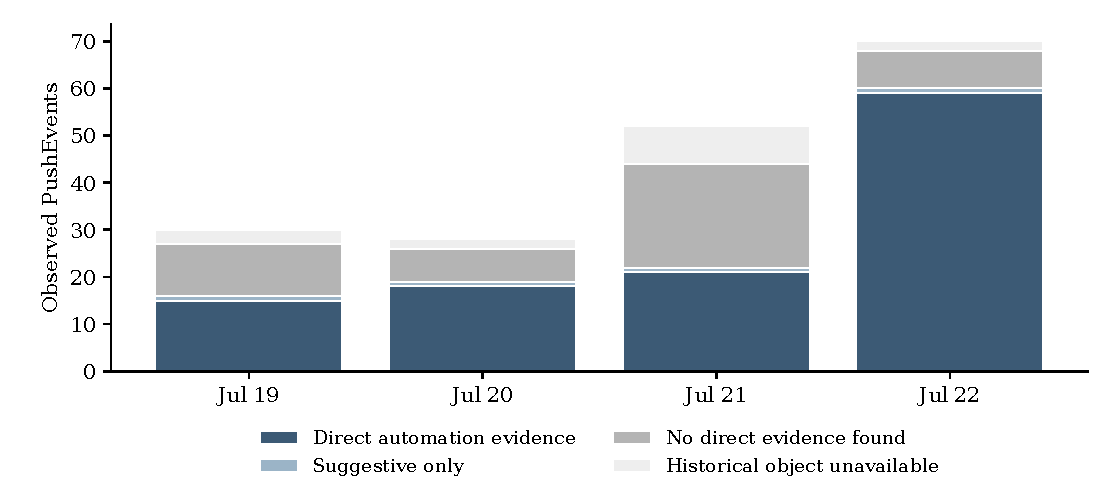
\includegraphics[width=\textwidth]{fig_evidence_automation.pdf}
\fignote{All 180 PushEvents on July 19--22 from the 40 core publishers. Classification concerns the head commit and available historical evidence. Direct evidence requires a machine identity corroborated by messages/files or a matching generating workflow; suggestive patterns and unavailable objects remain separate. No-direct-evidence cases are not certified human activity. Non-push primary events are omitted from this figure but retained in Table~\ref{tab:evidence_audit}.}
\end{figure}

\clearpage
{\footnotesize\setlength{\tabcolsep}{3pt}
\begin{longtable}{@{}p{.065\textwidth}rrp{.13\textwidth}p{.61\textwidth}@{}}
\caption{Individual review of every core-window publisher}\label{tab:evidence_cases}\\
\toprule Case & Events & Auto & Evidence & Basis and qualification \\
\midrule\endfirsthead
\toprule Case & Events & Auto & Evidence & Basis and qualification \\
\midrule\endhead
\bottomrule\endfoot
C002 & 4 & 4 & Direct & GitHub Actions author; generated snake SVG files. \\
C003 & 4 & 4 & Direct & readme-bot; scheduled WakaTime README workflow. \\
C006 & 1 & 0 & Not identified & Kubernetes/project files; no identified automated publishing mechanism. \\
C008 & 3 & 3 & Direct & readme-bot; historical scheduled WakaTime workflow. \\
C014 & 5 & 0 & Not identified & Build-fix commits; CI and stale-issue workflows do not establish automation of these pushes. \\
C021 & 5 & 0 & Not identified & IDE-file removals and a project README; no direct automation evidence. \\
C024 & 8 & 0 & Insufficient & Eight regularly timed profile-repository pushes, but historical objects unavailable; timing alone is insufficient. \\
C039 & 21 & 7 & Direct & Snyk bot heads; dependency-upgrade messages and manifests. \\
C043 & 16 & 16 & Direct & GitHub Actions author; generated snake SVG files. \\
C047 & 3 & 0 & Not identified & Favicon and application changes; no identified automatic publisher. \\
C049 & 10 & 0 & Not identified & Stack/queue exercises and React signup edits; repetitive messages alone do not establish automation. \\
C051 & 3 & 3 & Direct & readme-bot; historical scheduled WakaTime workflow. \\
C062 & 3 & 1 & Direct & Snyk bot head; lucide-react dependency upgrade. \\
C070 & 4 & 4 & Direct & github-actions identity; scheduled video-index pipeline and matching commit message. \\
C083 & 4 & 0 & Suggestive & Four 22:00 UTC host-list updates; an update-and-push script and example crontab exist, but deployment of that schedule is unverified. \\
C084 & 8 & 8 & Direct & github-actions[bot] author; generated deployment output, not inferred from the repository topic. \\
C089 & 4 & 4 & Direct & readme-bot; historical scheduled WakaTime workflow. \\
C093 & 6 & 2 & Direct & Snyk bot heads; mysql2 dependency upgrades. \\
C098 & 1 & 0 & Not identified & Engineering scripts/documents; no identified automatic publisher; commit title uses a local calendar date. \\
C099 & 3 & 0 & Not identified & HTML/CSS fitness-layout edits; no identified automatic publisher. \\
C110 & 2 & 1 & Direct & pyup-bot identity; Sphinx dependency update. \\
C115 & 3 & 1 & Direct & Snyk bot head; dependency-upgrade manifest changes. \\
C116 & 2 & 0 & Not identified & Application project-page edits; no identified automatic publisher. \\
C119 & 2 & 0 & Insufficient & Two CreateEvents only; no commit to inspect. Repository creation is not evidence of coding. \\
C123 & 1 & 0 & Not identified & Java generic-type examples; no identified automatic publisher. \\
C133 & 1 & 0 & Not identified & Three-line HTML change through GitHub UI; GitHub/web-flow is not itself bot evidence. \\
C139 & 7 & 0 & Not identified & Authentication and interface changes; no identified automatic publisher. \\
C140 & 4 & 0 & Mixed & Mixed activity: BibTeX edits and a merge; one onset commit is generated by github-actions[bot] and an exact historical import workflow. \\
C148 & 1 & 0 & Not identified & Power-system code repository; inspected core head resolves a gitignore conflict, not an automatic release. \\
C159 & 1 & 1 & Direct & readme-bot; historical weekly WakaTime workflow. \\
C161 & 7 & 7 & Direct & GitHub Actions author; generated snake SVG files. \\
C177 & 5 & 0 & Insufficient & Historical repository and four core heads unavailable. \\
C183 & 6 & 2 & Direct & Snyk bot heads; Dockerfile vulnerability-fix updates. \\
C222 & 10 & 0 & Not identified & C-sharp interview/data-structure exercises; the term Auto Stack is not evidence of a bot. \\
C226 & 1 & 0 & Not identified & README edits via GitHub UI; no identified automatic publisher. \\
C229 & 1 & 0 & Not identified & React router and page components; no identified automatic publisher. \\
C242 & 4 & 4 & Direct & GitHub Actions author; generated snake SVG files. \\
C260 & 12 & 0 & Not identified & Kotlin multiplatform examples; repeated init messages cover different files and do not establish automation. \\
C272 & 9 & 0 & Insufficient & Three core heads in two repositories unavailable; event combinations alone are insufficient. \\
C273 & 42 & 41 & Direct & All 41 core heads identify pyup-bot and change dependency requirements. \\
\end{longtable}}
\noindent\footnotesize Events counts all primary events on July 19--22; Auto counts only directly evidenced automated push heads. ``Not identified'' is not proof of manual authorship. Mixed denotes the account with a generated onset-authored commit alongside other activity; that generated commit is not itself a core push head. Case IDs map to account/repository/commit URLs and dated API evidence in \texttt{results/evidence\_20261020/individual\_case\_review.csv}. The review is AI-assisted and has not been independently validated by a second reviewer.\normalsize

